%% Copyright (c) 2004  SciSoft.  All rights reserved.
%%
%% This file is part of CGAL (www.cgal.org); you may redistribute it under
%% the terms of the Q Public License version 1.0.
%% See the file LICENSE.QPL distributed with CGAL.
%%
%% Licensees holding a valid commercial license may use this file in
%% accordance with the commercial license agreement provided with the software.
%%
%% This file is provided AS IS with NO WARRANTY OF ANY KIND, INCLUDING THE
%% WARRANTY OF DESIGN, MERCHANTABILITY AND FITNESS FOR A PARTICULAR PURPOSE.
%%
%% 
%%
%% Author(s)     : Fernando Cacciola <fernando_cacciola@hotmail.com>

\chapter{2D Straight Skeleton}
\label{chapter-straightskeleton2}

\section{Definitions}

\subsection{Simple Polygon}

A 2D \textbf{Simple Polygon} is a set of one or more simple contours. A 2D \textbf{Contour} is a sequence of 3 or more non-collinear (and non-coincident) vertices. A 2D \textbf{Vertex} is a 2D \ccc{Point}.\\
The vertices in a contour embeds 2D \textit{oriented straight line segments} called contour edges. A \textbf{Contour Edge} connects two consecutive vertices, and the cycle of edges in a contour is closed (i.e. there is an edge connecting the last and first vertices). A contour X is said to \textit{intersect} contour Y if any edge in Y intersects any edge in X; and a contour X is said to \textit{contain} contour Y if any vertex of Y is inside X.\\
Contours in a simple polygon must be arranged such that no contour intersects any other contour and exactly one contour, called the \textbf{Outer Contour}, contains the rest of the contours, called \textbf{Inner Contours} or \textbf{Holes}. The outer contour must be oriented counter-clockwise (CCW) while inner contours must be oriented clockwise (CW). Inner contours cannot be nested, that is, no inner contour can contain any other contour.

\subsection{Inward Offset Simple Polygon}

For any 2D Simple Polygon, called the \textbf{Source Polygon}, there can exist a \textit{set} of 0, 1 or more \textbf{Inward Offset Simple Polygons}, or just Offset Polygons for short, at some Euclidean distance \textit{t} $>0$. Any contour edge of such offset polygon, called an \textbf{Offset Edge} corresponds to \textit{some} contour edge of the source polygon, called its \textbf{Source Edge}. An offset edge is parallel to its source edge and has the same orientation. The Euclidean distance between the \textit{lines} supporting an offset edge and its source edge is exactly \ccc{t}.\\
An offset edge is always located \textit{to the left} of its source edge (which is an oriented straight line segment).\\
An offset polygon can have less, equal or more sides as its source polygon.\\
If the source polygon has no holes, no offset polygon has holes. If the source polygon has holes, any of the offset polygons can have holes itself, but it might as well have no holes at all (if the distance is sufficiently large).\\
Since any offset polygon is a simple polygon, its outer contour is oriented counter-clockwise while its holes (if any) are oriented clockwise.

\begin{figure}[htbp]
\begin{ccTexOnly}
\begin{center}
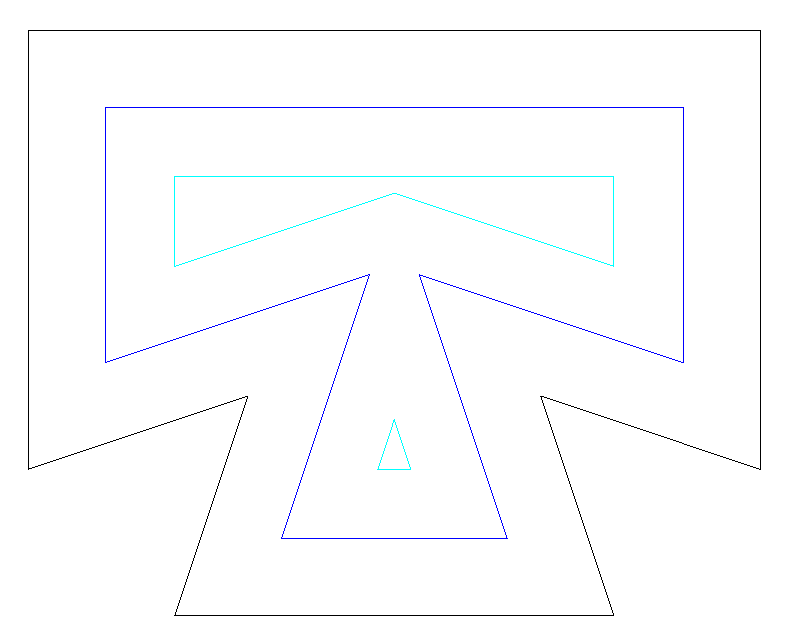
\includegraphics{fig0} % omit suffix .eps to supprt PS and PDF
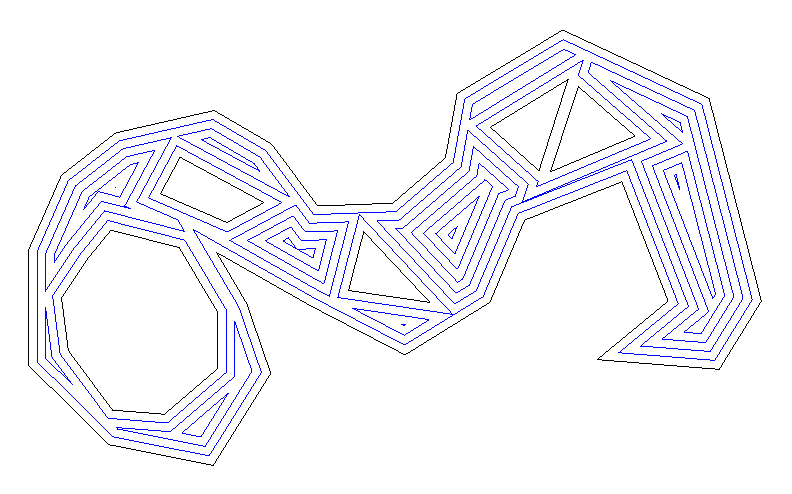
\includegraphics{fig1} % omit suffix .eps to supprt PS and PDF
\end{center}
\end{ccTexOnly}
\caption{Polygon with no holes and 2 inward offsets at distances 1 and 2 (Left) and polygon with holes and many inward offsets at various distances (Right)
\label{Simplepoly-offsets}}
\begin{ccHtmlOnly}
<TABLE CELLSPACING=40>
<TR>
<TD>
<CENTER>
<IMG BORDER=0 SRC="./fig0.png" ALIGN=center ALT="Polygon with no holes and 2 inward offsets">
</CENTER>
</TD>
<TD>
<CENTER>
<IMG BORDER=0 SRC="./fig1.png" ALIGN=center ALT="polygon with holes and many inward offsets at various distances">
</CENTER>
</TD>
</TR>
</TABLE>
\end{ccHtmlOnly}
\end{figure}

\subsection{Straight Skeleton of a 2D Simple Polygon}
 
The 2D \textbf{Straight Skeleton} of a simple polygon is a special partitioning of the polygon interior into \textbf{Straight Skeleton Regions} corresponding to the monotone areas traced by a continuous \textit{inward offsetting} of the contour edges. Each region corresponds to exactly 1 contour edge.\\
These regions are bounded by angular bisectors of the supporting lines of the contour edges and each such region is a non-convex simple polygon itself.\\
It was first introduced in:\\

@Article{,
author = {O. AICHHOLZER, F. AURENHAMMER, D. ALBERTS, BERND GARTNER},
title = {A Novel Type of Skeleton for Polygons}
}

\begin{figure}[htbp]
\begin{ccTexOnly}
\begin{center}
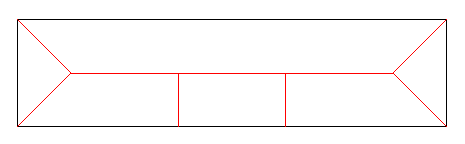
\includegraphics{fig2} % omit suffix .eps to supprt PS and PDF
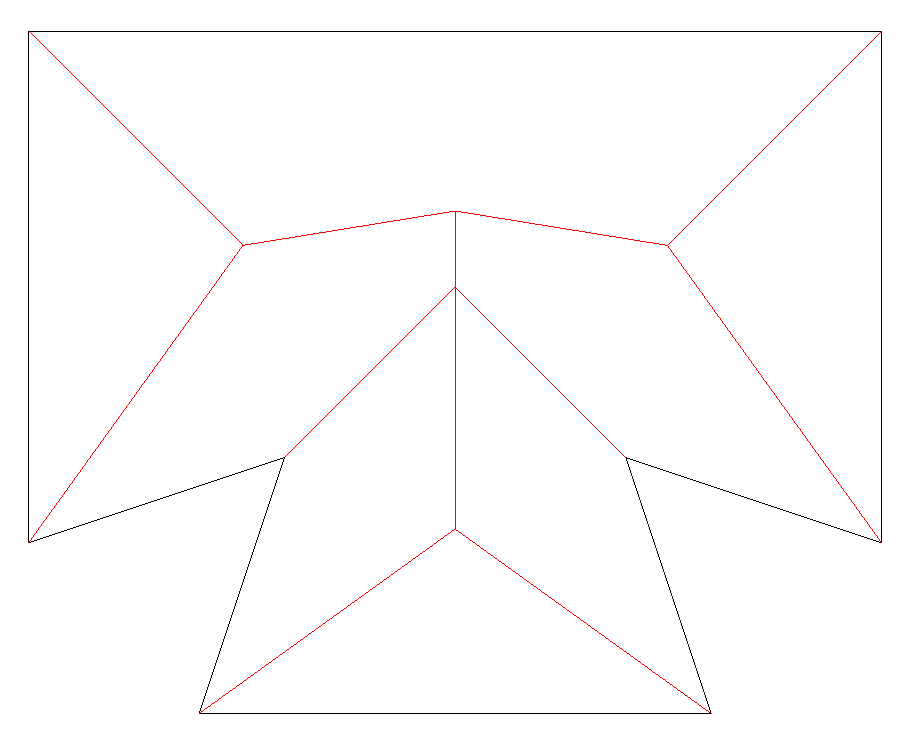
\includegraphics{fig3} % omit suffix .eps to supprt PS and PDF
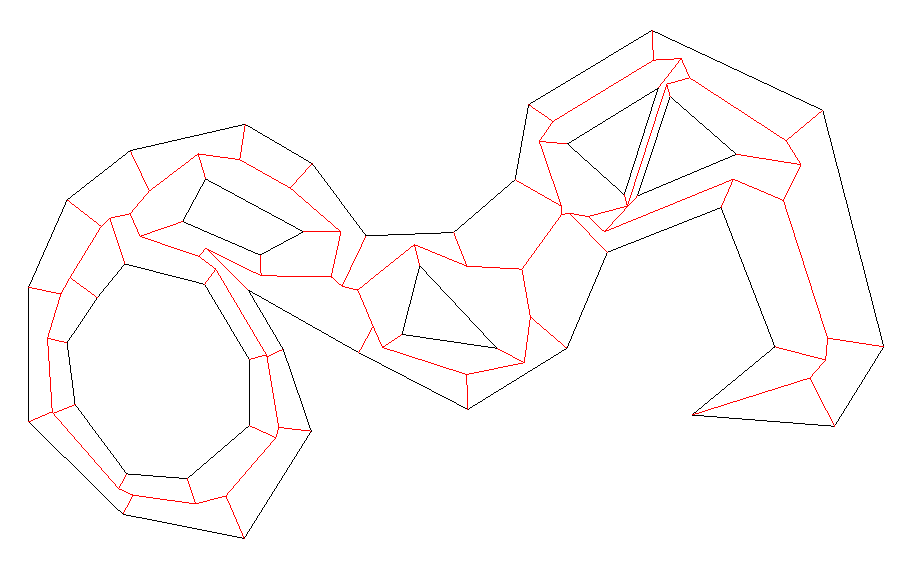
\includegraphics{fig4} % omit suffix .eps to supprt PS and PDF
\end{center}
\end{ccTexOnly}
\caption{Example straight skeletons
\label{SampleSLS}}
\begin{ccHtmlOnly}
<TABLE CELLSPACING=40>
<TR>
<TD>
<CENTER>
<IMG BORDER=0 SRC="./fig2.png" ALIGN=center ALT="Sample Skeleton 0">
</CENTER>
</TD>
<TD>
<CENTER>
<IMG BORDER=0 SRC="./fig3.png" ALIGN=center ALT="Sample Skeleton 1">
</CENTER>
</TD>
<TD>
<CENTER>
<IMG BORDER=0 SRC="./fig4.png" ALIGN=center ALT="Sample Skeleton 2">
</CENTER>
</TD>
</TR>
</TABLE>
\end{ccHtmlOnly}
\end{figure}
  
\subsubsection{Angular Bisecting Lines and Offset Bisectors}  

Two non-parallel lines, intersecting at a point, are bisected by two other lines passing through that intersection point.\\
Two parallel lines are bisected by another parallel line placed halfway in between.\\
Given just one line, any perpendicular line can be considered the bisecting line (any bisector of any two points along the single line).\\
The bisecting lines of two edges are the lines bisecting the supporting lines of the edges (if the edges are parallel or collinear, there is just one bisecting line)

The halfplane to the left of the line supporting a contour edge is called the \textbf{offset zone} of the contour edge.\\
Given any number of contour edges (not necessarily consecutive), the intersection of their offset zones is called their \textbf{combined offset zone}.

Any two contour edges define an \textbf{offset bisector}, as follows:
If the edges are non-parallel, their bisecting lines can be decomposed as 4 rays originating at the intersection of the supporting lines. Only one of these rays is contained in the combined offset zone of the  edges (which one depends on the possible combinations of orientations). This ray is the offset bisector of the non-parallel contour edges.\\
If the edges are parallel (but not collinear) and have opposite orientation, the entire and unique bisecting line is their offset bisector. If the edges are parallel but have the same orientation, there is no offset bisector between them.\\
If the edges are collinear and have the same orientation, their offset bisector is given by a perpendicular ray to the left of the edges which originates at the midpoint of the \textit{combined complement} of the edges. (The \textit{complement} of an edge/segment are the two rays along its supporting line which are not the segment and the \textit{combined complement} of N collinear segments is the intersection of the complements of each segment). If the edges are collinear but have opposite orientation, there is no offset bisector between them.

%% Figure of bisecting lines and offset bisectors here

\subsubsection{Faces, Edges and Vertices}

Each region of the partitioning defined by a straight skeleton is called a \textbf{Face}. Each face is bounded by straight line segments, called \textbf{Edges}. Exactly one edge per face is a \textbf{Contour Edge} (corresponds to a side of the polygon) and the rest of the edges, located in the interior of the polygon, are called \textbf{Skeleton Edges}, or \textbf{Bisectors}.

The Bisectors of the straight skeleton are segments of the \textit{offset bisectors} as defined previously. Since an offset bisector is a ray of a bisecting line of 2 contour edges, each skeleton edge (or bisector) is  uniquely given by two contour edges. These edges are called the \textbf{defining contour edges} of the bisector. 

The intersection of the edges are called \textbf{Vertices}. Although in a simple polygon, only 2 edges intersect at a vertex, in a straight skeleton, 3 edges intersect a any given vertex. That is, vertices in a straight skeleton have degree 3.\\
A \textbf{Contour Vertex} is a vertex for which 2 of its incident edges are contour edges.\\
A \textbf{Skeleton Vertex} is a vertex who's incident edges are all skeleton edges.

A \textbf{Contour Bisector} is a bisector who's defining contour edges are consecutive. Such a bisector is incident upon 1 contour vertex and 1 skeleton vertex and touches the input polygon at exactly 1 endpoint.\\
An \textbf{Inner Bisector} is a bisector who's defining contour edges are not consecutive. Such a bisector is incident upon 2 skeleton vertices and is strictly contained in the interior of the polygon.



\section{Representation}

This \cgal\ package represents a straight skeleton as a \ccc{Halfedge Data Structure} (HDS) whose \textit{vertices} embeds 2D Points.\\
Its \textit{halfedges}, by considering the source and target points, \textit{implicitly} embeds 2D \textit{oriented} straight line segments. 

A face of the straight skeleton is represented as a face in the HDS. Both contour and skeleton edges are represented by pairs of opposite HDS halfedges, and both contour and skeleton vertices are represented by HDS vertices.

In a HDS, a border halfedge is a halfedge which is incident upon an unbounded face. In the case of the straight skeleton HDS, such border halfedges are oriented such that their left side faces outwards the polygon. Therefore, the opposite halfedge of any border halfedge is oriented such that its left side faces inward the polygon.

The skeleton halfedges are oriented such that their left side faces inward the region they bound. That is, the vertices (both contour and skeleton) of a face are circulated in counter-clockwise order. There is one and only one contour halfedge incident upon any face. 

By requirement, a simple polygon must have the outer contour oriented CCW and the holes oriented CW. In the straight skeleton, these contours are traced by the \textit{border halfedges} (those facing outward) of the HDS, but in the opposite direction. That is, the vertices of the polygon's contours can only by traced from straight skeleton by circulating the border halfedges, and the resulting vertex sequence will be reversed w.r.t the input vertex sequence.

A skeleton edge, according to the definition given in the previous section, is defined by 2 contour edges. In the representation, each one of the opposite halfedges that represent a skeleton edge is associated with one of the opposite halfedges that correspond to one of its defining contour edges. Thus, the 2 opposite halfedges of a skeleton edge link it to its 2 defining contour edges.

Starting from any border contour halfedge, circulating the structure walks through border counter halfedges and traces the vertices of the polygon's contours (in opposite order).\\
Starting from any non-border but contour halfedge, circulating the structure walks through skeleton halfedges until the source contour halfedge is reached, and it traces the vertices (both contour and skeleton) of the face that corresponds to the source contour edge. Such a face is itself a non-convex simple polygon oriented CCW.

A vertex is the intersection of contour and/or skeleton edges. Since a skeleton edge is defined by 2 contour edges, any vertex is itself defined by a unique set of contour edges. These are called the \textbf{defining contour edges} of the vertex.\\
A vertex is identified by it's set of defining contour edges. Two vertices are distinct if they have differing sets of defining contour edges. \textit{Vertices can be distinct even if they are geometrically embedded at the same point}.
 
Contour vertices have exactly two defining contour edges, which are the contour edges incident upon the vertex; while skeleton vertices have exactly 3 defining contour edges.

The Euclidean distance from any vertex to the \textit{lines} supporting its defining contour edges is the same for all such lines (this is the distinctive characteristic of a straight skeleton). This distance is called the \textbf{time} of the vertex. Note that different vertices can have the same time. Contour vertices have time zero.

\begin{figure}[htbp]
\begin{ccTexOnly}
\begin{center}
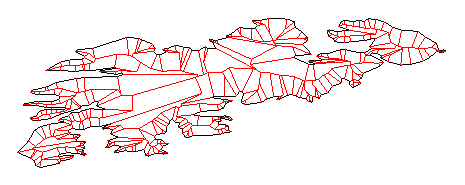
\includegraphics{fig5} % omit suffix .eps to supprt PS and PDF
\end{center}
\end{ccTexOnly}
\caption{Straight Skeleton Data Structure
\label{Simplepoly-offsets}}
\begin{ccHtmlOnly}
<TABLE CELLSPACING=40>
<TR>
<TD>
<CENTER>
<IMG BORDER=0 SRC="./fig5.png" ALIGN=center ALT="Straight skeleton DS">
</CENTER>
</TD>
</TR>
</TABLE>
\end{ccHtmlOnly}
\end{figure}

\section{API}

The Straight Skeleton data structure is encapsulated by any model of the \ccc{HalfedgeDS} concept.\\
The straight skeleton construction algorithm is encapsulated in the class \ccc{Straight_skeleton_builder_2<Gt,Ssds>} which is parameterized on a Geometric Traits (class \ccc{Straight_skeleton_builder_traits<Kernel>}) and the Straight Skeleton data structure (Ssds).

The polygon offset construction algorithm is encapsulated in the class \ccc{Polygon_offset_builder_2<Ssds,Gt,Container>} which is parameterized on the Straight Skeleton data structure (Ssds), a Geometric Traits (class \ccc{Polygon_offset_builder_traits<Kernel>}) and a Container type where the resulting offset polygons are generated.

To construct the straight skeleton of a simple polygon you must:
 
(1) Instantiate the straight skeleton builder.\\
(2) Enter one contour at a time, starting from the outer contour, via the method \ccc{enter_contour}. The input polygon must be strictly simple (non-intersecting) and there cannot be coincident or collinear vertices in the input (Keep in mind the definition and requirements of a Simple Polygon as expressed in the first section of this chapter).\\
(3) Call \ccc{construct_skeleton} once all the contours have been entered.\\

To construct an inward offset polygon you must:
 
(1) Construct the straight skeleton of the source polygon.\\
(2) Instantiate the polygon offset builder passing in the straight skeleton.\\
(3) Call \ccc{construct_offset_polygons} passing the desired offset distance and an output iterator that can store a \ccc{boost::shared_ptr} of \ccc{Container} instances (each representing one offset polygon) into a resulting sequence. Typically, you'll use a back insertion iterator for that.\\
Each element in the resulting sequence is a \ccc{boost::shared_ptr} holding a dynamically allocated instance of the Container type. Such a container can be any model of the \ccc{VertexContainer_2} concept, for example, a \ccc{CGAL::Polygon_2}, or just a \ccc{std::vector} of 2D points.

Both algorithms (for the construction of the straight skeleton and offset polygons) are highly sensitive to roundoff errors, therefore, they needs exact predicates to be reliable. Without exact predicates is almost certain that they will fail resulting in a straight skeleton or polygon offset topologically inconsistent (incomplete or non-planar). Fortunately, they don't need exact constructions.\\
The recommendation is to use a filtering kernel such as \ccc{Exact_predicates_inexact_constructions_kernel}.

\subsection{Example}

\ccIncludeExampleCode{../examples/Straight_skeleton_2/Straight_skeleton_2.C}

\section{Straight Skeletons, Medial Axis and Voronoi Diagrams}  

The Straight Skeleton of a simple polygon looks similar to the Medial Axis and the Voronoi Diagram of the polygon in the way it partitions the polygon; however, unlike the Medial Axis and Voronoi Diagram, the
bisectors are not equidistant to its defining edges but to the \textit{supporting lines} of such edges. As a result, Straight Skeleton bisectors might not be located in the center of the polygon and so cannot be regarded as a proper Medial Axis in its geometrical meaning.\\
On the other hand, only reflex vertices (whose internal angle $>pi$) are the source of deviations of the bisectors from its center location. Therefore, for convex polygons, the Straight Skeleton, the Medial Axis
and the Voronoi Diagram are \textit{exactly} equivalent, and, if a non-convex 
polygon contains only vertices of low reflexivity, the Straight Skeleton bisectors will be placed nearly equidistant to their defining edges, producing a Straight Skeleton pretty much alike a proper Medial Axis.

%% Straight Skeleton, Medial Axis and Voronoi Diagram figures here

\section{Straight Skeleton of a general figure in the plane}

A Straight Skeleton can also be defined for a general multiply-connected planar directed straight-line graph by considering all the edges as embedded in an unbounded region. The only difference is that in this case some faces will be only partially bounded.\\
This generalization was introduced in:

"Straight Skeletons for General Polygonal Figures in the Plane"\\
O. AICHHOLZER, F. AURENHAMMER

Unfortunately, the current version of this CGAL package can only construct the straight skeleton in the interior of a simple polygon; currently, it doesn't handle general polygonal figures in the plane.

% +------------------------------------------------------------------------+
%%RefPage: end of main body, begin of sfsooter
% EOF
% +------------------------------------------------------------------------+

